\par As described above, diKTat is very configurable and user-friendly. But these are not all of its advantages and features. Below will be presented and described unusual and important killer-features of diKTat.

\subsection{Configuration file}
\par
It's worth starting with the configuration file. This is a file in which the user can manually turn rules on and off or configure the rules settings. Below is one of the rules in the configuration file.


\begin{center}
\begin{tabular}{@{}l@{}}
 name: FILE\underline{ }IS\underline{ }TOO\underline{ }LONG\\ 
 \hspace{1cm}enabled: true\\
 \hspace{1cm}configuration:\\
 \hspace{2 cm}maxSize: '2000'\\
 \hspace{2 cm}ignoreFolders: ' '\\
\end{tabular}
\end{center}

Each rule in this file has 3 fields: name - the name of the rule, enabled - whether the rule is enabled or disabled (all rules are enabled by default), configuration - parameters for the rule. With the first two, everything is obvious. The third parameter is less obvious. The configuration is a set of "properties" to configure this rule. For example, for a rule "FILE\underline{ }IS\underline{ }TOO\underline{ }LONG", that checks the number of lines in a Kotlin file, the user can configure the maximum number of lines allowed in the file - by changing the "maxSize" in the configuration, or the user can specify paths to folders that do not need to be checked - by writing the path in "ignoreFolders". \\

\subsection{Create ASTNode}
\par
Another feature is a method that allows you to construct an abstract syntax node from text. This algorithm can parse the code even partially, when you do not need to save the hierarchy of the file (with imports/packages/classes).
For example it can parse and provide you a sub-tree for these lines of code:

\begin{lstlisting}[caption={Example of creating node.}, label={lst:example1}, language=Kotlin]
	val nodeFromText: ASTNode = KotlinParser().createNode("val age: Int = 21")
\end{lstlisting}

\tikzstyle{every node}=[draw=black,thick,anchor=west, scale = 0.5]
  
\begin{tikzpicture}[%
  grow via three points={one child at (0.3,-0.8) and
  two children at (0.3,-0.8) and (0.3,-1.5)},
  scale=0.5,
  edge from parent path={(\tikzparentnode.south) |- (\tikzchildnode.west)}]
    
  \node {PROPERTY}
    child { node {val}}
    child {node {WHITE\underline{ }SPACE}}
    child {node {IDENTIFIER}}
    child {node {COLON}}
    child {node {WHITE\underline{ }SPACE}}
    child {node {TYPE\underline{ }REFERENCE}
    	child {node {USER\underline{ }TYPE}
		child {node {REFERENCE\underline{ }EXPRESSION}
			child {node {IDENTIFIER}}
		}
	}
    }
    child [missing] {}
    child [missing] {}
    child [missing] {}  
    child {node {WHITE\underline{ }SPACE}}
    child {node {EQ}}
    child {node {WHITE\underline{ }SPACE}}
    child {node {INTEGER\underline{ }CONSTANT}
    	child {node {INTEGER\underline{ }LIRETAL}}
    };
\end{tikzpicture}

As you can see in the examples, we pass to the method the text of the source code that we want to transform and the flag, which is set to false by default. The flag should be set to true in order to immediately build a tree with a root node of the FILE type. What's going on inside this method? First of all, the system properties are set (for example: set "idea.io.use.nio2" to true). Further in the method, the text is checked. If the text of the code contains such keywords as import or package, then the method builds a tree with a root node of the FILE type, otherwise it tries with a different root type. In both cases, at the end, if the tree contains an ERROR\underline{ }ELEMENT type of node, it means that an error was made in the code and the method was unable to build the tree and, therefore, throws an exception.\\
This helps us to implement such complex inspections like the detection of commented code, helps easily fix the code without manually building sub-trees in visitors\\

\subsection{"SUPPRESS annotation"}
\par
What if the user wants one of the diKTat rules not to check a piece of code? The \textsl{SUPPRESS} annotation will help with this. This annotation can be supplied to ignore a certain rule. For instance, if run this code:

\begin{lstlisting}[caption={Function with incorrect name.}, label={lst:example1}, language=Kotlin]
	/**
* This is example
*/

package org.cqfn.diktat

/**
* Simple class
*/
class User(private val name: String, private val age: Int) {
	/**
	* Function with incorrect name
	* 
	* @return is username longer than age
	*/
	fun IsInCoRrEcTnAMe() = name.length > age
}

\end{lstlisting}

There will be warning: 
$$
\texttt{ \small{ $\big[$FUNCTION\underline{ }NAME\underline{ }INCORRECT\underline{ }CASE$\big]$  function/method name should be in lowerCamelCase}}
$$

But if there is a \textsl{@SUPPRESS} before this method, then there will be no errors at run.
\begin{lstlisting}[caption={Function with incorrect name, but with suppress.}, label={lst:example1}, language=Kotlin]
	/**
* This is example
*/

package org.cqfn.diktat

/**
* Simple class
*/
@Suppress("FUNCTION_NAME_INCORRECT_CASE")
class User(private val name: String, private val age: Int) {
	/**
	* Function with incorrect name
	* 
	* @return is username longer than age
	*/
	fun IsInCoRrEcTnAMe() = name.length > age
}

\end{lstlisting}

The example shows that the method has SUPPRESS annotation. Therefore, the \\ FUNCTION\underline{ }NAME\underline{ }INCORRECT\underline{ }CASE rule will be ignored on this method and there will be no error. The search method for a given annotation goes up recursively to the root element of type FILE, looking for the annotation. This means that Suppress can be placed not only in front of knowingly incorrect code, but also at the upper levels of the abstract tree. In our example, the annotation is not in front of the method, but in front of the class and still works. Also, you can put several annotations:
\begin{lstlisting}[caption={Function with incorrect name, but with suppress.}, label={lst:example1}, language=Kotlin]
@set:[Suppress("WRONG_DECLARATION_ORDER") Suppress("IDENTIFIER_LENGTH")]
\end{lstlisting}

\subsection{WEB}
\par
Also worth mentioning is the existence of a web version of diKTat.. This is a very handy tool that can be used quickly, and most importantly, it is very simple. The link can be found in or you can find it in "\nameref{sec:download}" chapter or in ktlint project as reference.\footnote{\url{https://github.com/pinterest/ktlint\#online-demo}}
\begin{figure}[H]
  \centering
  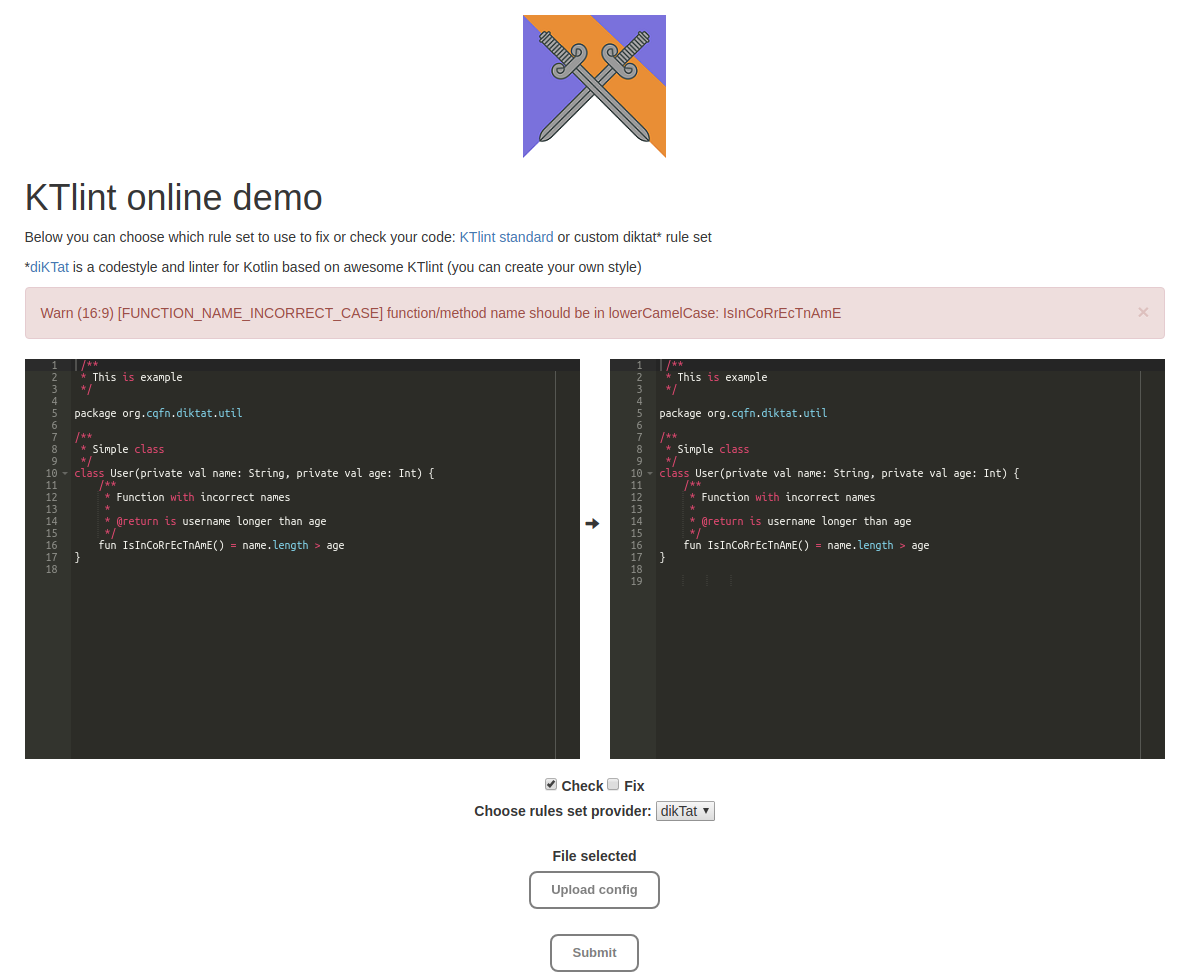
\includegraphics[scale=0.3]{pictures/web-example.png}
  \caption{Example of web application} 
\end{figure} 

\subsection{Validation rules}
\par
As it has been mention earlier, diktat has a highly customizable configuration file, but manually editing it is error-prone, for example, name of the rule can be incorrect due to a typo. Diktat will validate configuration file on startup and suggest the closest name based on \textsl{Levenshtein} method.

\subsection{CI-CD}
\par
One of the most important parts of open source project is CI/CD pipeline as it brings considerable benefits to the entire software development process. It improves code quality, customer satisfaction and reduces costs, including time, of making new features.